\chapter{Development Methodology}
\label{chap:developmentMethodology}
This section begins with a comparison between Waterfall development and agile development. Further is contains descriptions regarding the different development methodologies that have been brought up in discussion. Each subsection
includes both a short explanation, advantages and drawbacks for each methodology.

\section{Waterfall vs Agile development}
The first formal description of waterfall was published in a 1970 article by Winston W. Royce\cite{waterfall}. This method has been around for decades. The waterfall method is 
based on the idea of visiting each of the phases, Initiation, Analysis, Design, Construction, Testing, Implementation and Maintenance, only once and finish one before starting the next. The name is given from the idea of progress flowing through 
each phase, like a waterfall. This results in huge challenges regarding controlling dependencies if the project does reiteration over previous phases at a later stage.

Agile software development is not one certain method, but rather a group of software development methods based on iterative and incremental development. The concept of agile software development was introduced in The Manifesto for Agile Software Development, 2001\cite{agilemanifesto}. Even though iterative and incremental development methods had been around for some years, this manifesto gathered all best-practices in one place. The most used agile methods are, in no particular order, Extreme Programming, Adaptive Software Development, Feature Driven Development, Scrum, Kanban, Lean Software Development and Agile Unified Process. 

For the sake of this project, we chose to research waterfall, Scrum and Kanban in order to find a suitable development method.

\subsection{The Waterfall Method}
%%%%%%%%%%%%%%%%%%%%%%%%%%%
%Needs reference
Figure \ref{fig:waterfall} shows a graphical explanation of the sequential design process called the 
waterfall method.

The main advantage to the waterfall method is that bugs and changes are cheaper to 
fix if you fix them right away, as it will save you a lot of time and/or money later on.

The main drawbacks are that once the project has moved on to 
the next phase, the team should not backtrack and edit the previously completed 
phases, since this might make the further implementation more difficult. The fact 
that planning has to be done very thoroughly in the beginning to avoid having to 
reiterate previous phases at a later stage as this can be costly and complex, is 
also a disadvantage. Leading to a problem with projects where there is no overview 
to what is to be done and how long time it will take, this method will lead to 
uncertainty. A roll back to an earlier stage will most likely prove early estimates 
wrong and might cause complications to the development.

\begin{figure}
	\begin{center}
		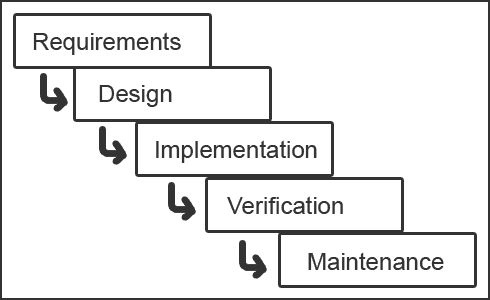
\includegraphics[width=10cm]{Pictures/waterfall_model}
	\end{center}
	\caption{Graphical representation of the waterfall method\cite{waterfallmodel}}
	\label{fig:waterfall}
\end{figure}

\subsection{Scrum}
\label{sec:scrum}
%%%%%%%%%%%%%%%%%%%%%%%%%%%%%%
% Needs reference
Figure \ref{fig:scrum} shows a graphical explanation of the Scrum method, one of many agile 
development methodologies. It is an iterative, incremental 
model which emphasizes on doing several short sprints where the goal is to complete 
some smaller set of tasks. After a given period of time, usually one to four weeks, the 
development team summarizes what have been done and what is left from the current 
sprint, which needs to be completed in the upcoming sprints.

The advantages of scrum is that it makes the software development more versatile, 
the team can work on all phases and parts of the project at the same time, and 
update earlier assumptions based on newer discoveries. Meaning that requirements and 
modelling does need to be finished before starting implementation and because of this, 
changes are less expensive to do. This is done by having a more relaxed relationship 
to documentation of source code and the process.

Nothing is written in stone until the product is done, as opposed to the waterfall 
method, mentioned earlier.

The main drawback of Scrum is the complexity of it. All methods has a certain learning 
curve at the beginning, leading to stress or less effective work. Scrum has several 
submethods, all with small differences. This may lead to a learning curve for 
experienced users.

A more specific explanation of how this project used Scrum is found in Section \ref{sec:sprints}.

\subsection{Kanban}
The Kanban is, as formulated by Anderson (2003\cite{Kanban}), a method for software development with an emphasis on just-in-time delivery, while maintaining focus on not overloading the developers. It emphasizes that developers pull work from a queue, and the process, from definition of a task to its delivery to the customer, is displayed for all other participants to see.

Kanban is based on some basic principles:
\begin{description}
	\item[Start with what you do now.] The method does not define a specific set of roles for team members, or process steps to follow. There is no such thing as "the Kanban software development process" or "the Kanban project management method". The method bases further work by starting with the roles and processes you have and stimulates continuous, incremental and evolutionary changes to your system.
	\item[Agree to pursue incremental, evolutionary change.] The organization (or team) must agree that continuous, incremental and evolutionary change is the way to develop improvements and make the changes stick. The Kanban method encourages continuous small incremental and evolutionary changes to your current system.
	\item[Respect the current process, roles, responsibilities \& titles.] It is likely that the organization currently has some elements that work properly and are worth bringing with for the future. By agreeing to respect current roles responsibilities and job titles we eliminate initial fear of change. This should enable the team to gain broader support for a Kanban initiative. 
\end{description}

\subsubsection{Core practices}
According to Anderson (2003\cite{Kanban}) there was originally five core practices in the Kanban method. 
\begin{itemize}
	\item \emph{Visualize.} A common way to visualize the work flow is to use a card wall with cards and columns. The columns representing the different states or steps in work flow. This is similar to a scrumboard.
	\item \emph{Limit WIP.} Limiting work-in-process implies that a pull system is implemented on parts or all of the work flow. The critical elements are that work-in-process at each state in the work flow is limited and that new work is "pulled" in when there is available capacity within the WIP limit of the team.
	\item \emph{Manage flow.} The flow of work through each state in the work flow should be monitored, measured and reported. By managing the flow continuously, the changes to the system can be evaluated to have positive or negative effects on the system.
	\item \emph{Make Policies Explicit.} Until the mechanism of a process is made explicit it is often hard to hold  a discussion about improving it. With an explicit understanding it is possible to move a more rational, empirical, objective discussion of issues. This is more likely to facilitate consensus around improvement suggestions. 
	\item \emph{Implement Feedback Loops.} Collaboration to review flow of work. Organizations that have not implemented the second level of feedback - the operations review - have generally not seen process improvements beyond a localized team level. As a result, they have not realized the full benefits of Kanban observed elsewhere.
\end{itemize}

\begin{figure}
	\begin{center}
		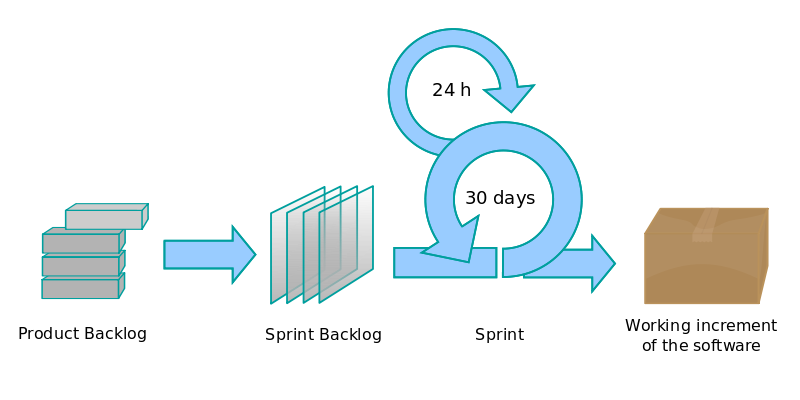
\includegraphics[width=14cm]{Pictures/Scrum_model}
	\end{center}
	\caption{Graphical representation of the SCRUM method\cite{scrummodel}}
	\label{fig:scrum}
\end{figure}

\section{Choice of methodology}
\label{sec:choiceofmethodology}
The development team chose the Scrum methodology instead of Kanban, due to 
several reasons. Foremost, the customer asked the team to work in an agile methodology, and preferably Scrum, since they could relate to Scrum. 
"We want the process to be as agile as possible, to a certain level. Waterfall will not 
suffice". The customer had many ideas regarding the layout and the functionality of the 
applications, and were not sure what to include. This leading to a situation where 
spending time making a detailed requirement specification and locking down all the 
details was pointless.

The customer was likely to make changes to the initial requirements once the first plan 
was ready. Secondly, the team was way more eager to try out an agile methodology rather than to use waterfall. 
In the choice between Kanban and Scrum, we lacked the proper knowledge to set those two apart, and had to do some extra investigation in order to fully understand what they meant. After reading about both Scrum and Kanban, the Kanban method did not make very much sense to us. 
The simple fact that Scrum is highly recommended by real-life developers, is a good 
argument for choosing Scrum over any other methodology. We were in the opinion that Scrum would suit our project the best, and therefore chose to use Scrum over the other methodologies.

\subsection{Sprints}
\label{sec:sprints}
This section gives a short description of how the Scrum development method was used in the project. 
For a general explanation of Scrum see Section \ref{sec:scrum}.

\subsubsection{Sprint duration}
We decided on having 14 day sprints. After discussions with the customer,
we agreed that this would be a suitable duration, due to the fact 
that the documentation needed for each sprint would be time consuming 
for shorter sprints.

\subsubsection{Sprint Planning Meeting}
To start each sprint, we held a sprint planning meeting. During this meeting, we discussed which user 
stories/epics from the sprint backlog should be worked on during the sprint. The reason behind such a 
meeting is to make sure the team is on updated on the goals for the following sprint. To decide what 
user stories/epics should be chosen, the priorities given by the customer was used as a pinpoint. If 
the customer wanted to make any changes during a sprint, the changes were noted and discussed during 
the next sprint planning meeting.

\subsubsection{Daily Standup}
The daily standups (also commonly known as daily scrum meeting) were held on Mondays, Wednesdays and 
Fridays. The team decided on this semi-daily recurrence since not all team members were able to work 
on the project every day. During the standup meetings all team members would answer three questions: 
what have you done since our last meeting, what will you work on until the next meeting, and what 
problems did occur since our last meeting?

Answering these questions gave a certain status update, and made it easier to re-assign team members 
to tasks if needed. During the standups all technical discussions were discouraged. If any technical 
questions arose, the people involved would discuss this after the meeting, to make sure they were not 
wasting other people's time. Each standup had a max allowed length of 15 minutes. 

\subsubsection{Sprint retrospective}
The sprint retrospective is the written conclusion of the sprint. A meeting was held at the end of each 
sprint, discussing the results throughout the sprint, both finished and unfinished tasks. The tasks not 
completed were moved to the next sprint, and the reason for the task not being completed was stated in 
the sprint report. 

The sprint report also includes an update of the sprint backlog, along with an overview of how much time 
was spent on each task, making it easy to compare to the time estimate. 

The sprint retrospective also contains a burndown chart, giving a visual representation of how the team 
worked during the sprint.

For each sprint we answered the following questions: 
\begin{itemize}
	\item What went well?
	\item What shall we start doing?
	\item What could have gone better?
	\item What should we stop doing?
\end{itemize}
%TODO: the questions

\subsubsection{Explanation of Sprint Backlog}
The sprint backlog is a task management tool to document and ensure the progress of the sprint. Each task the 
team chooses to focus on in the sprint is enlisted. The task is given an ID and already has a name. The 
Function number is an hour-independent number telling how difficult the team expects the task to be. The 
base number represents how many hours the team expects to work to finish one story point. The base number multiplied 
with the function number for a task gives the estimated work hours needed to finish a task.

The base number may change from sprint to sprint, but not during a sprint. The team did an evaluation of 
the base number in advance of each sprint, to make good estimates.

The name column is used to keep track of who is responsible for the task. This may change during the sprint, 
but the sprint backlog should always be showing the correct info.

Based on how many team members are available and how many work hours they may put in, the team gives an 
expected decrease of the story points left. This is reflected in the sprint burndown chart for each sprint, 
as a straight decreasing line.